
\documentclass{report}

\usepackage[utf8]{inputenc}
\usepackage[portuges]{babel}
\usepackage{graphicx}
\graphicspath{{img/}}
\usepackage[normalem]{ulem}
\usepackage[left=3cm,top=4cm,right=2cm,bottom=3cm]{geometry}
\title{\textbf{Mestrado Integrado em Engenharia Informática}\\\textbf{Processamento de Linguagens}\\ 2º Trabalho Prático}
\author{Francisco Oliveira (a78416)\\Raul Vilas Boas (a79617)\\Vitor Peixoto (a79175)}
\date{\today}

\begin{document}
\maketitle
\tableofcontents


% Introdução
\chapter{ Introdução
}
No âmbito da unidade curricular de Processamento de Linguagens, 
foi-nos pedido que, baseado em Markdown, 
criássemos uma linguagem semelhante e uma ferramenta em Flex 
capaz de tranformar esta notação mais leve em \LaTeX. 
\\
Neste relatório será explicado o processo de desenvolvimento 
e as decisões tomadas ao longo da realização do trabalho.

\chapter{ Requisitos
}
Neste trabalho foram pedidos vários requisitos principais, os quais falaremos em breve, 
contudo, tomamos iniciativa de adicionar algumas funcionalidades extra, com intuito 
de aprofundarmos o nosso conhecimento e aprendizagem neste tópico.
\\
Passamos agora a mostrar os requisitos em causa:

\section{ Principais
}
Foi-nos pedido que a nossa ferramenta fosse capaz de:
\begin{itemize}
\item  Criar vários níveis de títulos
\item  Formatar o texto para:
    \begin{itemize}
\item  Negrito
    \item  Itálico
    \item  Sublinhado
    \end{itemize}
\item  Criar listas de tópicos:
    \begin{itemize}
\item  Não-numerados
    \item  Numerados
    \item  Tipo entrada de dicionário 
    \end{itemize}
\end{itemize}

\section{ Extras
}
Ainda como extras, a nossa ferramenta é capaz de:
\begin{itemize}
\item  Texto rasurado
\item  Aceitar alguns comandos especiais:
    \begin{itemize}
\item  Footnote \footnote{{footnote}}
    \item  Comentários %Este é um comentário
    \item  Inserir novo parágrafo e quebra de página
    \item  Inserir imagens
    \end{itemize}
\end{itemize}


% Header tipo Chapter. Nao disponivel em artigos
\chapter{Demonstração
}

\section{Níveis de títulos
}
A nossa linguagem permite a utilização de todos os 
níveis de títulos existentes no \LaTeX. 
\\
Neste caso "Demonstração" seria um exemplo de título do tipo \textit{Chapter} 
e "Níveis de títulos" um tipo \textit{Section}. 
\\
Neste caso, o título deste capítulo "Demonstração" seria um exemplo 
de título do tipo \textit{Chapter} e "Níveis de titulos" um tipo \textit{Section}. 
O título de cada nível deve ser sempre indicado no início de uma nova linha, 
seguindo de “\#”, sendo que o número de ocorrências de “\#” indicam o nível do 
título (i.e. “\#” indica \textit{Chapter}, “\#\#” indica \textit{Section} e por aí adiante).
\\
Para além disto, há a opção de adicionar ou não numeração ao título, 
bem como o seu aparecimento no índice. Os títulos que não devem ser numerados 
nem indexados devem seguir-se de um “*” após todos os “\#”.
\\
Na imagem abaixo, pode-se compreender melhor o funcionamento 
do processo explicado acima:

\subsection{Exemplo de título SubSection
}
Temos ainda \textit{SubSubSection}, \textit{Paragraph}, \textit{SubParagraph}, 
bem como todos os anteriormente referidos títulos na sua versão 
com * (asterisco).
\subsection*{Exemplo de título SubSection*
}
Exemplo.

\begin{figure}[h]
	\centering
	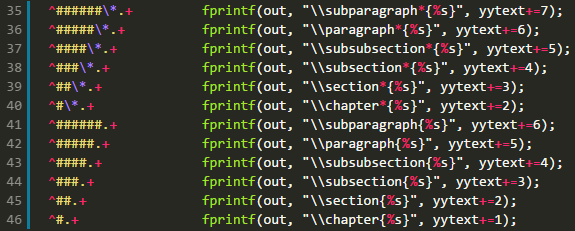
\includegraphics[scale=0.7]{titulos_flex.png}
	\caption{Código Flex - títulos}
\end{figure}

\begin{figure}[h]
	\centering
	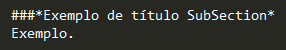
\includegraphics[scale=1]{titulo_source.png}
	\caption{Exemplos de títulos}
\end{figure}

\newpage

\section{Formatação de texto
}
Para os diferentes tipos de formatação são usados os seguintes estilos:
\begin{itemize}
\item  "*" para texto bold;
\item  "/" para texto itálico;
\item  "\_" para texto sublinhado;
\item  "\textasciitilde" para texto rasurado.
\end{itemize}
Este são apenas marcadores de inicio de formatação.
\\
Para além disso, o estado \textit{formating}, utilizado para sabermos 
que estamos dentro de uma formatação, não é exclusivo o que permite 
que qualquer texto possa ser introduzido dentro da formatação 
bem como formatações adicionais, como será demonstrado.

\begin{figure}[h]
	\centering
	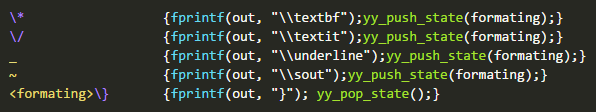
\includegraphics[scale=0.9]{formatacao_flex.png}
	\caption{Código Flex - Formatação}
\end{figure}


\subsection{Texto exemplo
}
Portanto como pedido, a nossa linguagem é capaz de acomodar texto em \textbf{bold}, 
em \textit{itálico}, \underline{sublinhado}, \sout{rasurado} bem como qualquer combinação entre eles. 
\\
Por exemplo \textbf{\textit{\underline{\sout{MAIS}}}} 
\footnote{{ texto em bold+itálico+sublinhado+rasurado}}

\begin{figure}[h]
	\centering
	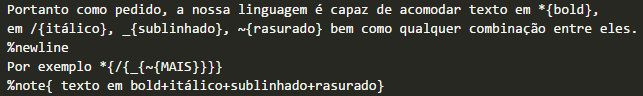
\includegraphics[scale=0.9]{formatacao_source.png}
	\caption{Exemplos de formatação de texto}
\end{figure}


\newpage

\section{Listas
}
Outro dos requisitos era a capacidade de criar listas.
Permitimos a criação de todos os tipos de listas pedidos, 
bem como listas aninhadas podendo estas ser ou não do mesmo tipo.
\\
Para criar uma qualquer lista deve-se utilizar as seguintes expressões:
\subsection{Listas não numeradas
}
\begin{itemize}
\item  "\textgreater\textgreater*"  para iniciar uma nova Lista não numerada
    \begin{itemize}
\item  "\textgreater\textgreater*"  para iniciar uma sub Lista não numerada
    \item  "\textgreater*" para continuar uma Lista não numerada
    \end{itemize}
\end{itemize} 
\subsection{Listas numeradas
}
\begin{enumerate}
\item  "\textgreater\textgreater\textit{dígito}\footnote{{um qualquer dígito}}" para iniciar uma nova Lista numerada
    \begin{enumerate}
\item  "\textgreater\textgreater\textit{dígito}" para iniciar uma sub Lista numerada
    \item  "\textgreater\textit{dígito}" para continuar uma Lista numerada
    \end{enumerate}
\end{enumerate}
\subsection{Entradas tipo dicionário
}
\begin{description}
\item[Exemplo]  "\textgreater\textgreater[\textit{palavra}]" para iniciar uma nova Entrada tipo dicionário
    \begin{description}
\item[NovoExemplo]  "\textgreater\textgreater[\textit{palavra}]" para iniciar uma nova Entrada tipo dicionário   
    \item[SubExemplo]  \textgreater[\textit{palavra}]" para continuar uma Entrada tipo dicionário
    \end{description}
\end{description}
Aqui temos alguns exemplos.

\begin{figure}[h]
	\centering
	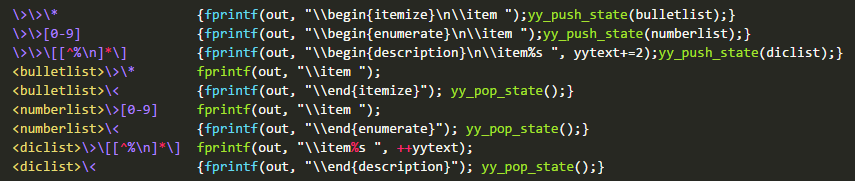
\includegraphics[scale=0.7]{listas_flex.png}
	\caption{Código Flex - Listas}
\end{figure}


\newpage

\subsection{Listas aninhadas
}
Apresentamos aqui um exemplo com várias listas aninhadas, 
e algumas delas formatadas.
\begin{enumerate}
\item  Alínea 1
    \begin{itemize}
\item  Ponto 1
        \begin{description}
\item[Palavra 1]  \textit{Significado 1 itálico}
        \end{description}
    \item  \textbf{Ponto 2 bold}
    \end{itemize}
\item  \underline{Alínea 2 sublinhado}
    \begin{itemize}
\item  Ponto 2
        \begin{enumerate}
\item  Alínea 2.1 rasurado
            \begin{itemize}
\item  \textbf{\textit{\underline{\sout{Ponto 2.1 bold+itálico+sublinhado+rasurado}}}}
            \end{itemize}
        \end{enumerate}
    \end{itemize}
\item  Alínea 3
    \begin{description}
\item[Palavra 1]  Significado 1
        \begin{enumerate}
\item  \sout{Alínea 3.1 rasurado}
        \end{enumerate}
    \item[Palavra 2]  Significado 2
        \begin{itemize}
\item  Alínea 3.2 
        \end{itemize}
    \end{description}
\end{enumerate}

\begin{figure}[h]
	\centering
	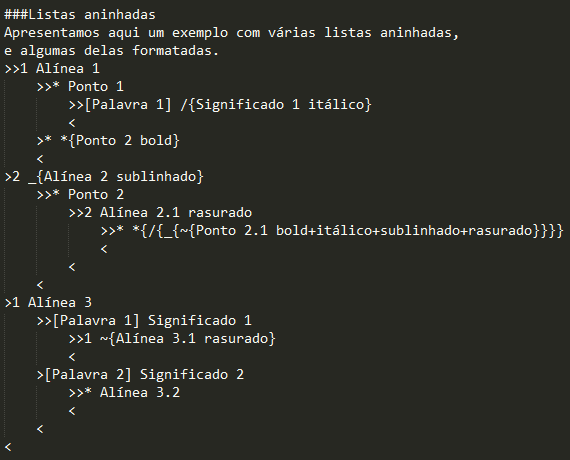
\includegraphics[scale=0.8]{listas_source.png}
	\caption{Exemplos da formatação de listas}
\end{figure}


\newpage

\section{Extras
}
Para além do que era pedido, fizemos ainda alguns extras. 
Primeiramente temos a \textit{footnote} 
\footnote{{texto rasurado também era um extra mas já foi falado}} 
que permite adicionar pequenas anotações ao texto, 
utilizando um simples comando \%note\{texto da nota\}. 
\\
Temos tambem comentários, comandos para inserir novas linhas, 
novo parágrafo e novas páginas.
\\
% COMENTARIO
Podemos também adicionar imagens e efetuar transformações, 
tais como alterar o tamanho da imagem, 
bem como adicionar uma legenda.
\\
Para adicionar uma imagem é necessário começar com [\textit{dígito}] 
que será a escala a que a imagem será representada (escala entre 0.0 e 9.9). 
Depois da escala deve introduzir o caminho até à imagem, 
usando para tal o comando [\textit{caminho}]. 
Finalmente há a hipótese de adicionar uma legenda usando 
(\textit{legenda}) após o caminho.

\begin{figure}[h]
	\centering
	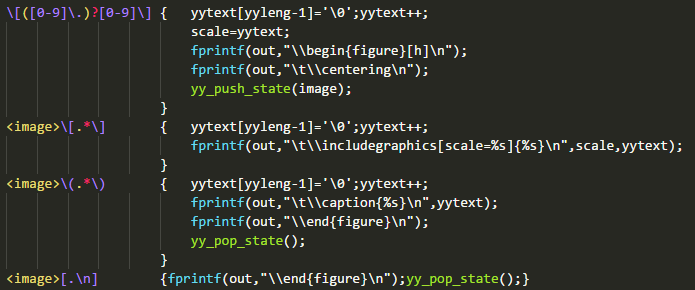
\includegraphics[scale=0.9]{imagem_flex.png}
	\caption{Código Flex - Imagem}
\end{figure}

\begin{figure}[h]
	\centering
	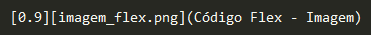
\includegraphics[scale=1]{imagem_source.png}
	\caption{Exemplo de formatação de imagems}
\end{figure}


\chapter{Conclusão
}
Este trabalho permitiu consolidar a matéria lecionada 
nas aulas da unidade curricular, mas também obter um maior 
conhecimento acerca do funcionamento do Flex, 
para além de permitir praticar o uso deste tipo de ferramentas 
para resolver problemas de conversão de linguagem, entre outros.
\\
Em suma, avaliamos a nossa prestação na resolução deste trabalho, como positiva.


\end{document}
